\documentclass[12pt]{article}
% Margin fixes
\oddsidemargin -0.5in
\evensidemargin -0.5in
\textwidth 7.25in
\topmargin 0.0in

\headheight 0.0pt
\headsep 0.0pt
\voffset 0.0pt
\textheight = 9.0in
\usepackage{amsmath,amssymb,graphicx,float}

\title{Michelson Interferometer}
\author{Nathan Grouse\\Lisa Tran}

\newcommand{\eV}{\text{eV}}
\newcommand{\V}{\text{V}}
\newcommand{\A}{\text{A}}

% Start the document!
\newcommand{\documentname}{\textsl{Article}}
\begin{document}
\maketitle

\section{Introduction}
\indent \indent Using the Michelson interferometer, one can measure the wavelength of a light source, the index of refraction of a material, and the width of a specral line.

\subsection{Apparatus}
\indent \indent Light from some source is directed at a beam splitter, oriented at 45 degrees with respect to the source. The beam splitter is coated on one side so that 50 percent of the indicident light is reflected while the other half is transmitted. The transmitted light is reflected by a mirror $M_1$ while the reflected light is reflected again by another mirror $M_2$. The two beams formed converge - constructively or destructively depending on the optical path length - to form a third beam which falls on a screen. The laser is a He-Ne laser with 5 selectable wavelengths. A vacuum chamber of some length L, in which air can be pumped out, is also used.

\begin{figure}[H]
\centering
\hspace{-0.0in}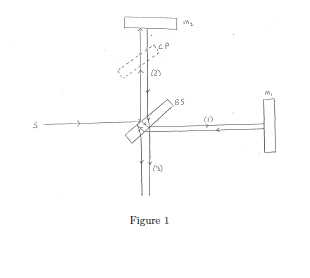
\includegraphics[scale=0.90]{apparatus.png}
\end{figure}

\section{Theory}
\indent \indent If the optical path length (OPL) for two beams seperated orignally from one beam from points A to B is the same, these beams constructively interfere (Duh). If The difference between the path lengths is half the wavelength, the beams destructively interfere. \\

\indent It's given that:
\[ 2D = N\lambda \]
\[ \lambda = \frac{2D}{N} \]

\indent Where N is the number of fringes that pass a fixed point when the OPL of one of the beams is changed by 2D. the mirror is moved some distance D, but the beam must approach and reflect from the mirror, moving through twice that distance. The number of times a fringe passes a fixed point determines the number of times the OPL was changed by one wavelength, thus the total change in OPL divded by the number of wavelengths in that change will give the change in OPL for just one wavelength. \\

\indent To calculate the index of refraction of air using a vacuum tube which slowly allows air to leak in, this equation is given:

\[ 2(n_a_i_r - 1)L = N\lambda \]

\indent This implies that $2(n_a_i_r)L$ is the difference in OPL from initial vacuum conditions to final air filled tube.

\[ \Delta OPL = OPL_f - OPL_i \]
\[ OPL_f = 2\int n \,ds = 2nL\]
\[ OPL_i = 2\int \,ds = 2L\]
\[\Delta OPL = 2(n-1)L = N\lambda \]

\indent Where we include a factor of 2 in front of the integral because the beam passes through the vacuum tube twice - before and after reflection.

\section{Data}
\begin{figure}[H]
\centering
\hspace{-0.0in}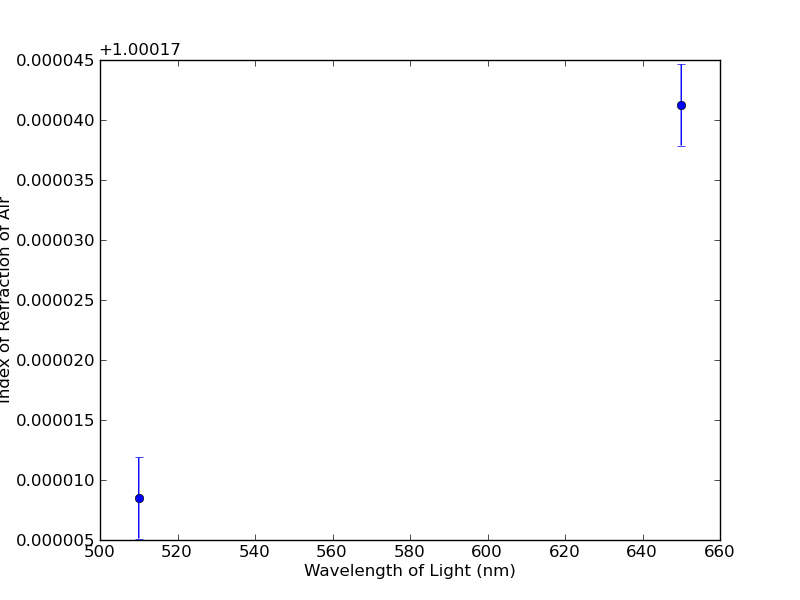
\includegraphics[scale=0.60]{Plot1.png}
\end{figure}

\section{Calculations}
\[n_a_i_r = \frac{N_g_r_e_e_n\lambda_g_r_e_e_n}{2L}+1 = \frac{(56 \frac{\Delta OPL}{\lambda})(5.10 x 10^-7 m)}{(2)(.08 m)}+1 = 1.0001785 \]
\[n_a_i_r = \frac{N_r_e_d\lambda_r_e_d}{2L}+1 = \frac{(52 \frac{\Delta OPL}{\lambda})(6.50 x 10^-^7 m)}{(2)(.08 m)}+1 = 1.00021125 \]

\section{Error Analysis}
\indent \indent Approximate values for the wavelengths of green and red light are used because of an inability to complete that section of the lab. Uncertainty in the length of the vacuum and fringe reading was determined by the precision of a ruler our ability to view a mark inbetween two fringes. The distance between ticks on the ruler was .1 cm, so it could be read accurately somewhere around $\pm .05 cm$. We could see our mark for fringe readings inbetween any two given fringes, so we assumed a maximum uncertainty of $\pm 1 fringe$ . Finding how uncertainty propogates in a quotient:
\[\frac{\delta q}{|q|} = \sqrt{(\frac{\delta x}{x})^2 + (\frac{\delta y}{y})^2 } \]

\indent There will only be uncertainty in the first term describing $n_a_i_r$, $\frac{N\lambda}{2L}$:
\[\delta q_g_r_e_e_n = (1.0001785 - 1)\sqrt{(\frac{.0005 m}{.08 m})^2 + (\frac{1 fringe}{56 fringes})^2 } = 3.377 x 10^-^6 \]
\[\delta q_r_e_d = (1.00021125 - 1)\sqrt{(\frac{.0005 m}{.08 m})^2 + (\frac{1 fringe}{52 fringes})^2 } = 4.212 x 10^-^6 \]

\indent The refractive index of air at 30 degrees celcius is 1.00026337. //

\indent Percent Errors:
\[\frac{|1.00026337 - 1.0001758|}{1.00026337} = .008 \% \]
\[\frac{|1.00026337 - 1.00021125|}{1.00026337} = .005 \% \]

\section{Conclusion}
\indent \indent The number I obtained is both reasonable and consistent with the accepted value. I did not see what I expected to see in terms of the first and qualitative half of the experiment. We were unable to generate - or at least recognize - circular or non-circular fringes.

\section{Questions}
\indent \indent 1. Were you able to discern any dispersion for air? \\
\indent I don't think so - not noted or remembered. \\
\indent 2. To observe white light fringes, you must use a compensating plate. Why? \\
\indent The manuel says its only possible to see white light frignes if the OPLs for the two arms are almost exactly same. A compensating place makes the OPLs for the beams equal when the distances $d_1$ and $d_2$ from the BS to each mirror respectively are equal. \\
\indent 3. Could you devise a way to measure the inex of refration of a transparent solid? \\
\indent Using the same apparatus and positioning as was used for the vacuum tube, place the transparent solid in an oven - capable of melting that solid - which allows for the entry and exit of a beam of light. Start counting fringes when the oven is turned on and use the same method to calculate the index of refraction of the solid:
\[ \Delta OPL = 2(n_s_o_l_i_d - n_a_i_r)L_o_v_e_n = N\lambda . \]

\end{document}